\chapter{Implementation}

[Beschreibung der Implementierung\footnotemark auf Basis des Entwurfs und der Methodologie / der geplanten Vorgehensweise zur Probleml\"osung im Kontext der Anforderungen. Hier ist Raum f\"ur Listings, wie z.B. das nun Folgende:


\footnotetext{Beachten Sie bei der Implementierung und deren Dokumentation bitte Clean Code Empfehlungen (vgl. hierzu z.B. \autocite{martin2008}).} 

\begin{lstlisting}[caption={Ein Beispiel: Hello World (JavaScript)}]
const helloWorld = "Hello, world!"
console.log(helloWorld)
\end{lstlisting}

Umfangreicher Quell-Code sollte in den Anhang ausgelagert werden.]

\section{Object Models}
  \label{impl_model}

In this chapter, the specific implementation of the object models described in \autoref{subsection:model} will be discussed. 

  \subsection{Validation Rule}
    \label{impl_model:rule}

    The subsection describes the implementation of the \verb;ValidationRule; object model as a TypeScript interface.

    \subsubsection{Retry Strategy}
      \label{impl_model:rule__retry}

      The \verb;retryStrategy; attribute of the validation rule model is very specific to the implementation of the FDS. The FDS is using a library called \emph{Got}\footnote{\emph{Got} is a Node.JS library to make HTTP requests. GitHub repository: \url{https://github.com/sindresorhus/got}.} to make HTTP requests to the external endpoints. Got provides the functionality to retry a failed HTTP request out of the box\footnote{For more information on Got's retry options, please refer to \url{https://github.com/sindresorhus/got/blob/main/documentation/7-retry.md}.}.

      The \verb;retryStrategy; attribute of a validation rule is a subset of the retry options provided by Got's retry API, and will be passed to the Got instance when the HTTP request is made for the corresponding rule evaluation. 

    \subsubsection{TypeScript interface}
      As the implementation of the model defined in \autoref{fig:uml_validation_rule}, a TypeScript interface is created to provide a clear structure of a validation rule.

      \begin{lstlisting}[style=es6, caption={TypeScript interface of a validation rule (TypeScript)}]
export interface ValidationRule {
  retryStrategy?: RetryStrategy | null
  requestUrlParameter?: GenericObject
  requestHeader?: GenericObject
  skip: boolean
  requestBody?: GenericObject
  condition: Condition | BooleanCondition
  method: "GET" | "PUT" | "POST" 
  failScore: number
  endpoint: string
  priority: number
  name: string
}

type GenericObject = { [key: string]: any } // Dictionary
type Condition = {
  path: string
  operator: OperatorType
  type: ConditionType
  value: any
  failMessage: string
}

type BooleanCondition = {
  all: Condition[]
} | {
  any: Condition[]
}

type RetryStrategy = {
  limit: number
  statusCodes: number[] 
}
      \end{lstlisting}

  \subsection{Validation Result}
  
    A TypeScript interface is created as the implementation of the validation result structure listed on \autoref{fig:uml_validation_result}. The FDS is not responsible in storing validation results in a database. Therefore, a Prisma schema won't be created for validation results. 

    \newpage
    \begin{lstlisting}[style=es6, caption={TypeScript interface of a validation result (TypeScript)}]
export interface Validation<T> {
  validationId: string
  fraudScore: number
  totalChecks: number
  runnedChecks: number
  skippedChecks: string[]
  additionalInfo: ValidationAdditionalInfo<T>
  events: ValidationEvent[]
}

export type ValidationEventStatus = "NOT_STARTED" | "FAILED" | "PASSED" | "RUNNING"
export type ValidationEvent = {
  name: string
  status: ValidationEventStatus
  dateStarted: string | null
  dateEnded: string | null
  messages?: string[]
}

export type ValidationAdditionalInfo<T> = {
  startDate: string
  endDate?: string
  customerInformation?: T
}
    \end{lstlisting}
\section{View}

  This chapter discusses the implementation of the features on the user interface described in \autoref{sub:design_view}.

  \subsection{Navigation}
  
    The user interface contains functionalities for several use cases, merged into a single web application. In a web application, routing plays a key role in determining what to show the user based on the URL address entered on the browser. Specifically in this case, routing can help in categorizing the current context of the application that consists of several views for different use cases. The following routes are implemented in the UI:

    \begin{itemize}
     \item Home page (path: \verb;/;)
     \item Create a new rule (path: \verb;/rules/new;)
     \item Edit a rule (path: \verb;/rules/<ruleName>;)\footnote{\emph{<ruleName>} refers to a dynamic value of a rule's name. Please take a look into \url{https://router.vuejs.org/guide/essentials/dynamic-matching.html} for more information.}
     \item List of rules (path: \verb;/rules;)
     \item Create a new validation (path: \verb;/validations/create;)
     \item See validation progress for specific validation ID (path: \verb;/validations/:validationId;)
     \item List of validations (path: \verb;/validations;)
    \end{itemize}
    
    To help the user in navigating the UI, a header is created and displayed on every page of the application. The header includes three buttons (\textsc{Home, Rules} and \textsc{Validations}), that links the user to the corresponding view of the application. 

    \begin{figure}[!ht]
     
\includegraphics[width=\textwidth]{images/ss_navigation.jpeg}
     \caption{Screenshot of the header to navigate the UI}
    \end{figure}

  \subsection{Rule Management Form}
  
    The rule management form is a reusable form, can be used to both create a new and edit an existing validation rule. The rule management form displays all the attributes of a \verb;ValidationRule; model as a form field. 

    \begin{figure}[!ht]
      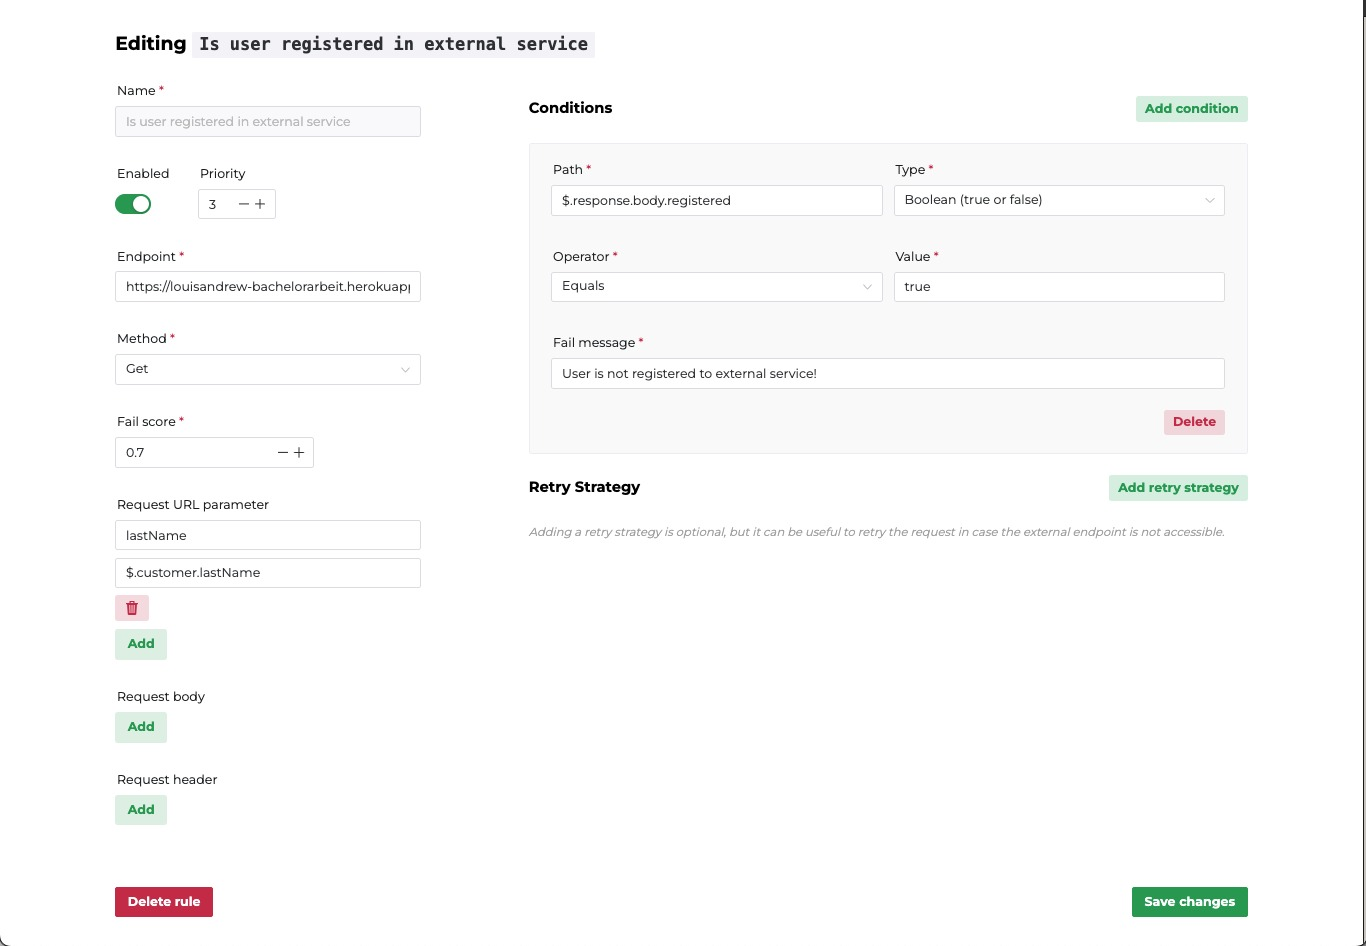
\includegraphics[width=\textwidth]{images/ss_sample_filled.jpeg}
      \caption{Screenshot of the rule management form}
    \end{figure}

    \subsubsection{Conditions Section}

      The \textsc{Conditions} section is a component, used to add one more condition to a validation rule. The \textsc{Conditions} section renders the list of conditions provided in a card, containing form fields for each attribute of the particular condition. Each card represents a single form, which also contains validation on its fields. 
      
      As mentioned before, the available values for the \verb;operator; attribute of a condition depends on its \verb;type; attribute. To prevent an invalid condition being sent to the FDS, the \textsc{Operator} field is a select field, and its options are defined by the current value inputted on the \textsc{Type} field. The intention of the restriction is to make sure that the \verb;operator; chosen is always valid to the corresponding \verb;type; of the condition.

      \begin{lstlisting}[style=es6, caption={Function to get list of available operators based on a condition's type attribute (TypeScript)}]
const getAvailableOperators = (type: ConditionType) => {
  switch (type) {
    case "string":
      return [
        { label: "Equals", value: "eq" },
        { label: "Starts with", value: "starts" },
        { label: "Includes", value: "incl" },
        { label: "Ends with", value: "ends" },
      ]
    case "number":
      return [
        { label: "Greater than", value: "gt" },
        { label: "Greater than equals", value: "gte" },
        { label: "Lesser than", value: "lt" },
        { label: "Leser than equals", value: "lte" },
        { label: "Equals", value: "eq" },
      ]
    case "array":
      return [
        { label: "Includes", value: "incl" },
        { label: "Excludes", value: "excl" },
        { label: "Number of items equals", value: "len" },
        { label: "Is empty", value: "empty" },
      ]
    case "boolean":
      return [{ label: "Equals", value: "eq" }]
    default:
      return []
  }
}
      \end{lstlisting}

      \begin{figure}[!ht]
        \centering
        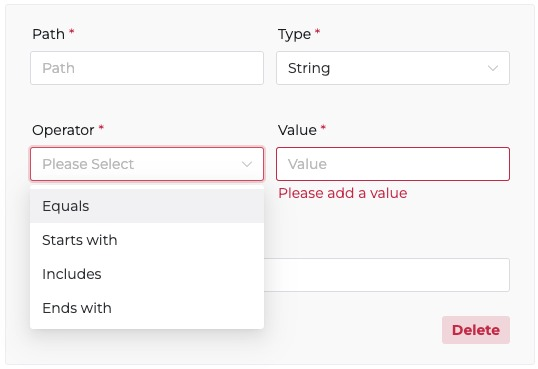
\includegraphics[width=0.8\textwidth]{images/ss_condition_op.jpeg}
        \caption{Screenshot of the "Operator" select field options, based on the current "Type" value}
      \end{figure}
      
      If more than one condition is provided, a radio field is also rendered, so that the user can choose one of the provided modifier for the list of conditions (either \textbf{\emph{ALL}} or \textbf{\emph{ANY}}). 

      A form validation is also implemented in the \textsc{Conditions} section. The validation not only make sure that all the required fields are filled, but also the value of the fields itself. For example, the validation will display an error message if the \textsc{Type} field is set to "Number", but the input value of the \textsc{Value} field is not a valid number. 

    \subsubsection{Autocomplete Input}

    A JSONPath expression is a valid value for some attributes of a \verb;ValidationRule;, and it also might be needed to access the current runtime information during a validation process, such as the HTTP response from the external endpoint, runtime secrets and customer information. Unfortunately, it might be difficult to memorize the expressions needed to access certain values, and it might also confuse the user. 

    \begin{figure}[!ht]
      \centering
      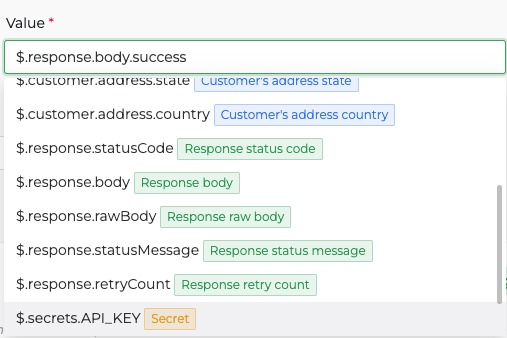
\includegraphics[width=0.5\textwidth]{images/ss_autocomplete.jpeg}
      \caption{Screenshot of the autocomplete input usage}
    \end{figure}

    To solve this problem, an autocomplete input field is provided in certain fields where a JSONPath expression is used. User can then display a list of possible JSONPath expressions by prefixing an input field with "\$", and choosing one of the expressions listed. User can also extend the expression chosen. The autocomplete input is used in the following form fields:

    \begin{itemize}
      \item \textsc{Path} field on \textsc{Conditions} section
      \item \textsc{Value} field on \textsc{Conditions} section
      \item Value field of a dynamic input\footnote{Autocompletion on \emph{\$.response} is not available here.}
    \end{itemize}

  \subsection{Validation Form}

    The validation form is a simple form similar to a customer registration form, specifically to mimic a new customer registration and to run a validation process directly after a new registration. Form validation is also implemented in the validation form to make sure that the customer information sent to the FDS is complete. A set of sample customers with specific characteristic is created to provide the functionality of pre-filling the validation form. 

    \begin{figure}[!ht]
      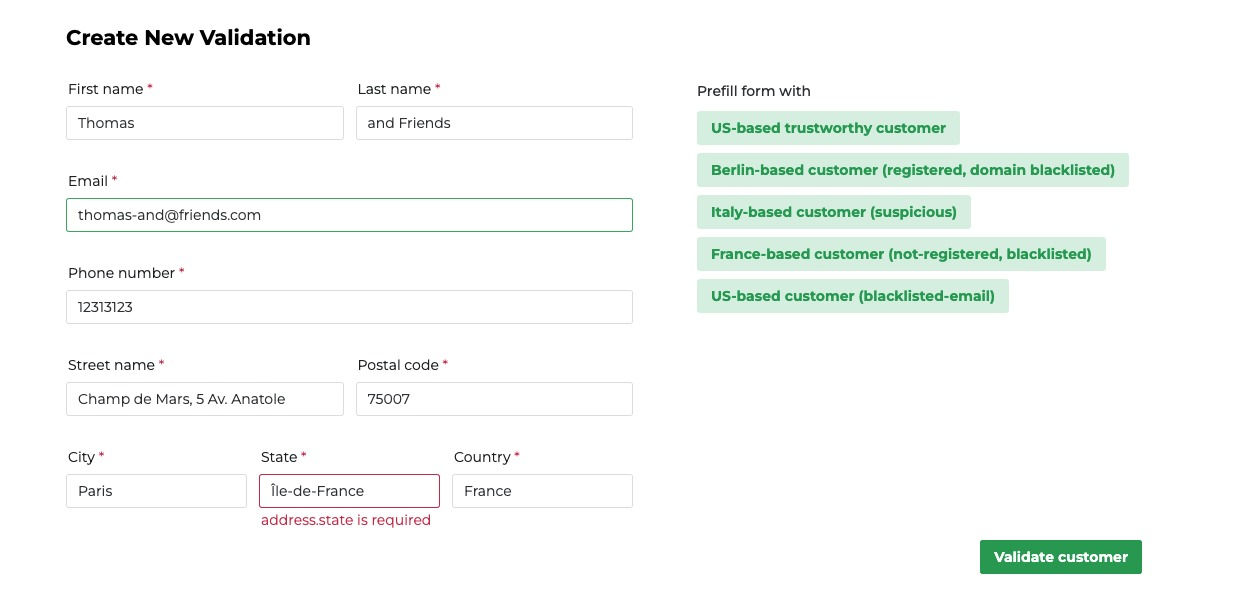
\includegraphics[width=\textwidth]{images/ss_customer_form.jpeg}
      \caption{Screenshot of the validation form}
    \end{figure}

    \begin{lstlisting}[style=es6, caption={Prefilling form values with a sample customer data (TypeScript)}]
const applySampleCustomer = (sampleCustomer: Customer) => {
  Object.assign(formValues, {
    ...sampleCustomer,
  })
}
    \end{lstlisting}

    When the user filled the fields properly and clicked the \textsc{Validate customer} button, the UI sends an HTTP POST request to the FDS with the customer data as the payload to schedule a new validation process. As the FDS returns an ID of the validation process, the UI will then redirect the user to the validation progress page, showing the validation progress in real time. 

    \begin{lstlisting}[style=es6, caption={ (TypeScript)}]
const { data } = await createNewValidation(customer)
if (data.validationId) {
  router.push(`/validations/${data.validationId}`)
}
    \end{lstlisting}

  \subsection{Validation Progress}
  
    To receive the real time event stream sent by the FDS as described in \autoref{impl_sse}, the \verb;EventSource; API can be used on the client side. With the \verb;EventSource; API, a persistent connection to the FDS will be opened, and the messages sent will be received by the client in real time. Because the FDS sends the messages as a string in an event stream, the UI has to parse the message content into a valid JSON object before processing it. 

    \begin{lstlisting}[style=es6, caption={Using the EventSource API in the browser (TypeScript)}]
const source = new EventSource(url)

source.onmessage = messageEvent => {
  try {
    const data = JSON.parse(messageEvent.data)
    // Do data processing
  } catch {
    // Handle error, if the message data is not a valid JSON object
  }
}
    \end{lstlisting}

    It is also important to close the connection to the event stream when it's no longer needed. The logic of closing the open connection when user leaves the current page is also implemented on the UI. 

    As the content of the message is parsed and identified as a valid \verb;ValidationResult; object, it is saved into the current state of the \verb;Validation; component, which renders the events of a validation process into a timeline component to give the user a better graphical overview of the current process. Vue3 uses the \emph{Proxy}\autocite[pp. 207-217]{gamma-1995} design pattern under the hood to provide a reactivity system on the UI, providing the possibility to update the timeline component every time a new validation result is published by the FDS. 

    \begin{figure}[!ht]
      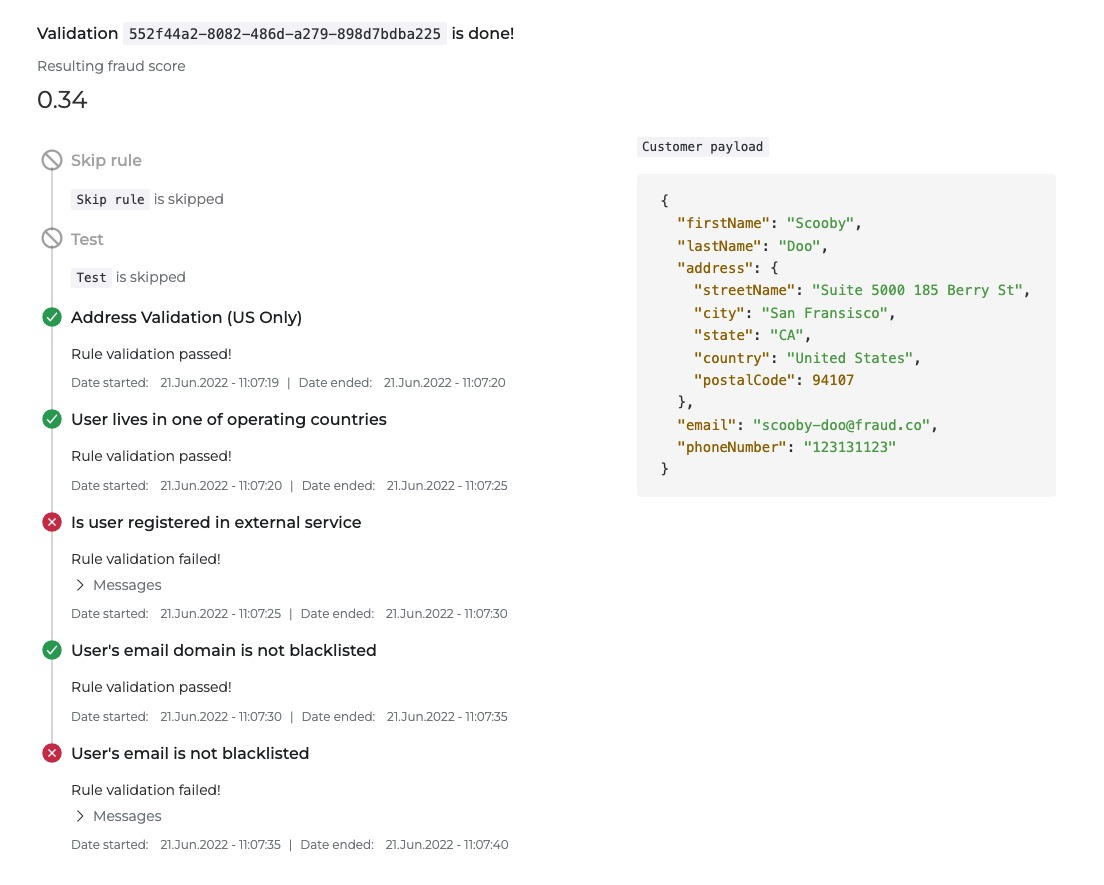
\includegraphics[width=\textwidth]{images/ss_validation_progress.jpeg}
      \caption{Screenshot of the validation progress in real time}
    \end{figure}

    The ID of the validation as well as the current fraud score of a validation process are always displayed, to give detailed information to the user regarding the current validation process. Additionally, the customer data is also displayed as a JSON object, to give the user with technical knowledge a better overview on the data being sent to the FDS. 
  
  \subsection{Runtime Secrets}

    A component to display a list of the available runtime secrets in a dialog is also created. For security purposes, only the key of the secrets are displayed within the component. The component also provides a possibility to create a new runtime secret and to delete an existing secret. User can create a new secret by clicking on the \textsc{Create a new secret} button, and adding the essential information on the form fields displayed. To delete an existing secret, a \textsc{Delete} button is displayed next to each secret's key name. The list of available runtime secret keys are also accessible on the autocomplete options, making it easier for the user to access the appropriate secret key without having to memorize the key name.
    
    \begin{figure}[!ht]
      \centering
      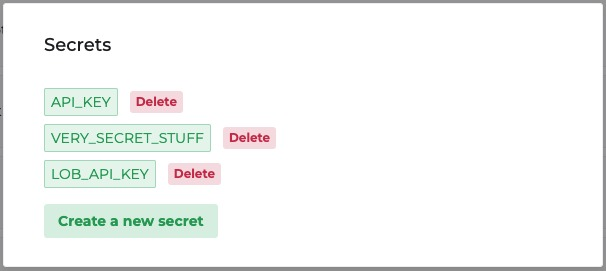
\includegraphics[width=0.6\textwidth]{images/ss_secrets.jpeg}
      \caption{Screenshot of a component to list available runtime secrets}
    \end{figure}
    
\section{Controller}

  This chapter describes the implementation of the features elicited on the previous chapters in details, specifically within the FDS component. All the HTTP routes of the FDS will be prefixed with \verb;/api/v1;.

  \subsection{Customer Validation on a Registration Event}

    An HTTP endpoint will be implemented to provide the possibility to schedule a validation process as soon as a new customer is registered. The endpoint should accept the customer information on the request body and return validation ID and additional information of the validation process as a response. Listed below is the code snippet of the HTTP controller of the endpoint to schedule a validation process:

    \begin{lstlisting}[style=es6, caption={HTTP controller of an endpoint to schedule a validation process (TypeScript)}]
// fds/src/routes/validation/validationController.ts

// Picks the `validationId` and `additionalInfo` attributes from `Validation` 
type ValidationSchedule = Pick<Validation, "validationId" | "additionalInfo"> 
     
@Route("validate")
@Tags("Validation")
export class ValidationController extends Controller {
  @SuccessResponse(201, "Validation started")
  @Response<ValidationErrorJSON>(422, "Validation Failed")
  @Response<WentWrong>(400, "Bad Request")
  @Post()
  public async validateCustomer(
   @Body() requestBody: Customer
  ): Promise<ValidationSchedule | WentWrong> {
    const result = await ValidationService.scheduleRulesetValidation(requestBody)
    const { data, error } = result

    if (error) {
      this.setStatus(400)
      return {
        message: error.message,
        details: error.details || "",
      }
    }

    return data
  }
} 
    \end{lstlisting}
    
    The HTTP controller is intentionally kept as simple as possible. The logic behind the process to schedule a validation is done by the \verb;ValidationService; and \verb;ValidationEngine; (discussed in \autoref{sub:process}). The \verb;ValidationService; is responsible in this particular case to get the lists of existing validation rules and runtime secrets (discussed in \autoref{sub:secrets}), then creating a new instance of \verb;ValidationEngine; as well as scheduling a new validation process. 

    \begin{lstlisting}[style=es6, caption={ValidationService schedule validation implementation (TypeScript)}]
// fds/src/routes/validation/validationService.ts

export class ValidationService {
  static async scheduleRulesetValidation(
    customer: Customer
  ): Promise<ApiResponse<ValidationSchedule>> {
    const { data: ruleset, error } = await RulesService.listRules()
    const secrets = await SecretsService.listSecrets()
    if (error) {
      return {
        data: null,
        error,
      }
    }

    const { validationId, additionalInfo } = await new ValidationEngine<Customer>()
      .setRuleset(ruleset)
      .setSecrets(secrets)
      .scheduleRulesetValidation(customer)

    return {
      data: {
        validationId,
        additionalInfo,
      },
      error: null,
    }
  }
}
    \end{lstlisting}

  \subsection{Validation Process}
    \label{sub:process}

    \subsubsection{Validation Process Flow}
    
      A validation process is started by iterating through a list of validation rules, making an HTTP request to the external endpoint listed on each rule and evaluating its response in comparison to the conditions attached on the rule. If the HTTP response from the external matches the conditions of the rule, the rule evaluation will be considered as a passed evaluation, otherwise it is a failed evaluation. The result of each rule evaluation determines the value of the resulting fraud score. The resulting fraud score will be calculated as follows: 

      \begin{itemize}
        \item Initialize an empty list of fraud scores. The list will be filled later with float numbers ranging between 0 and 1
        \item Go through the list of validation rules and run evaluation
        \item If the evaluation passed, append \verb;0; to the list of fraud scores
        \item Otherwise, append the validation rule \verb;failScore; attribute's value to the list of fraud scores
        \item At the end of the iteration, the list size should equal to the amount of available\footnote{\emph{Not skipped.}} validation rules
        \item The resulting fraud score is the sum of the scores in the list, divided by the number of available validation rules
      \end{itemize}
      
      In summary, the flow of a validation process will be represented by the flow diagram below:

      \begin{figure}[!ht]
        \centering
        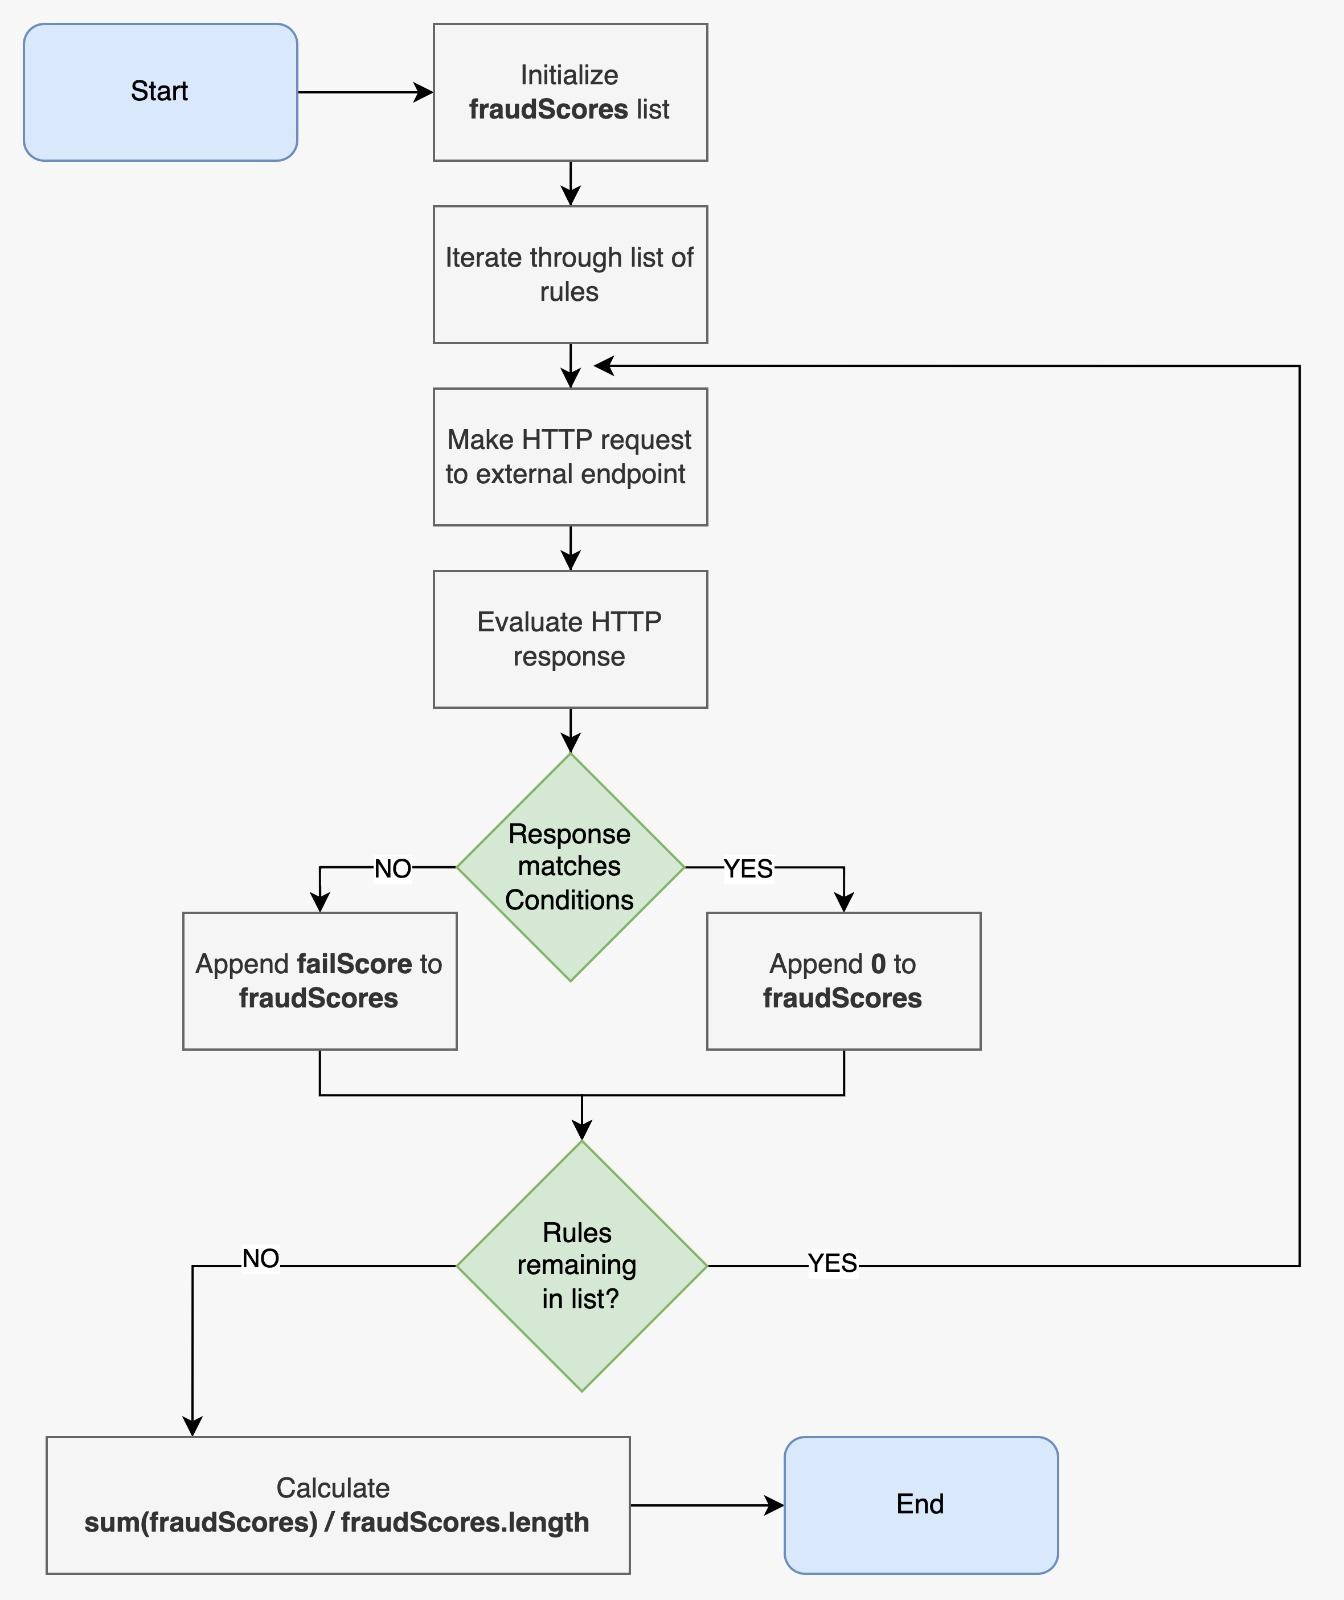
\includegraphics[width=0.8\textwidth]{diagrams/flow_validation_process.jpeg}
        \caption{Flow diagram of a validation process}
        \label{fig:flow_validation}
      \end{figure}
      
      The flow listed above will be executed by creating a \verb;ValidationEngine; instance and calling a public \verb;secheduleRulesetValidation; method. Before running a validation process, the list of validation rules as well as runtime secrets should be provided to the engine. The \verb;ValidationEngine; class uses method chaining\footnote{\emph{Method chaining} is a method to provide the possibility of invoking multiple method calls of an object without having to store an intermediary result in an additional variable.} as well as the \emph{Builder} design pattern discussed in \autocite[pp. 97-106]{gamma-1995} for its construction, to make the public API of a validation engine as simple as possible.

      \begin{lstlisting}[style=es6, caption={ValidationEngine class and the scheduleRulesetValidation method (TypeScript)}]
// fds/src/engine/valdiationEngine.ts
export class ValidationEngine<T> {
  private secrets: GenericObject = {}
  private ruleset: ValidationRule[] = []

  setSecrets(secrets: GenericObject) {
    this.secrets = secrets
    return this
  }

  setRuleset(ruleset: ValidationRule[]) {
    this.ruleset = [...ruleset.sort((a, b) => b.priority - a.priority)]
    return this
  }

  async scheduleRulesetValidation(data: T): Promise<Validation<T>> {
    if (this.ruleset.length === 0) {
      throw new Error("Ruleset is not set")
    }

    await this.constructValidationObject(data) // Construct a validation result
    this.validateRuleset(data)

    return this.validationResult
  }

  async validateRuleset(data: T): Promise<Validation<T>> {
    if (this.ruleset.length === 0) {
      throw new Error("Ruleset is not set")
    }

    if (!this.validation) {
      await this.constructValidationObject(data)
    }

    for await (const rule of this.ruleset.filter(({ skip }) => !skip)) {
      const evaluationResult = await this.evaluateRule(rule, data)
      await this.reviewEvaluationResult(evaluationResult, rule)
    }

    await this.afterValidation()

    return this.validationResult
  }
}
      \end{lstlisting}

    \subsubsection{Accessing Data by Evaluating JSONPath Expressions}
      
      To be able to access essential information stored in the current runtime scope a validation process, a JSONPath expression can be used in certain attributes of a validation rule. The provided runtime information of a validation process includes the customer information, runtime secrets and during a condition evaluation, the HTTP response from the external endpoint of the particular rule. 

      The ability to access certain information from the runtime scope is needed when an HTTP request is made and during the evaluation of a condition. To evaluate a JSONPath expression, the \verb;jsonpath; library is used. 

      \begin{lstlisting}[style=es6, caption={Accessing runtime information using JSONPath expression (TypeScript)}]
import jp from "jsonpath"

const accessDataFromPath = (runtimeData: any, expression: any) => {
  if (typeof expression !== "string") {
    return expression // A valid JSONPath expression is a string
  }
  
  try {
    const [dataFromPath] = jp.query(runtimeData, expression)
    if (!dataFromPath) {
      // Expression is valid, but the path doesn't point to a specific value
      return expression 
    }

    return dataFromPath
  } catch {
    return expression // The expression is either not a valid JSONPath expression
  }
}
      \end{lstlisting}

    \subsubsection{Making an HTTP Request to External Endpoints}

      A dedicated class (\verb;Agent;) is created to make an HTTP request to the external endpoint. The class will provide a layer of abstraction on top of the Got library that is being used to actually make the HTTP requests. 
      
      The class will also help in setting the request body, request header as well as to change the variables on the \verb;endpoint; attribute with its corresponding values. The class follows the \emph{Singleton} design pattern described in \autocite[pp. 127-134]{gamma-1995}, as there might only one instance needed for the whole application. The class is also implemented using the dependency injection in mind, for an easier access to the underlying library during the testing phase. The dependency injection is implemented by providing a \verb;context; object to the \verb;Agent; class beforehand. During runtime, the \verb;context; object contains a Got instance, used to make HTTP requests. In testing environment, the \verb;context; object contains a mocked Got instance.

      \begin{lstlisting}[style=es6, caption={Usage of the singleton pattern and dependency injection in Agent class (TypeScript)}]
export class Agent {
  private static context: Context // Dependency injection

  private static get client() {
    return Agent.context.client // `client` object is a Got instance
  }

  static setClient(context: Context) {
    this.context = context
  }
}
      \end{lstlisting}

    \subsubsection{Operators}

      \verb;Operators; are special classes that define the operation of a certain condition during a validation process. Each \verb;Operator; is grouped by its type and has two main properties \verb;identifier;, and \verb;operateFunction;
      
      The \verb;identifier; property of an operator refers to the operator's name, unique on its group of type. The \verb;identifier; attribute of an operator will be passed into the \verb;operator; attribute of a condition to describe the specific operator to be used in evaluating the particular condition. The \verb;operateFunction; attribute of an operator is a function that accepts two arguments, and returns a boolean value that indicates whether the operation is successful. An additional validation process is also implemented using the \verb;validateFunction; property to make sure that the value being passed into the \verb;operate; function of an operator is valid. The \verb;identifier; and \verb;operateFunction; attributes of an operator are passed into the object constructor during its initialization, while the \verb;validateFunction; attribute of an operator is defined by each subclass of the operator, grouped by its type.  
      
      \begin{lstlisting}[style=es6, caption={NumberOperator example (TypeScript)}]
export class NumberOperator extends Operator<number, NumberOperatorIds> {
  const validateFunction = (value) =>
    typeof value === "number" &&
    !isNaN(parseFloat(`${value}`))
}

export const numberOperators: Record<NumberOperatorIds, NumberOperator> = {
  eq: new NumberOperator("eq", (a, b) => b === a),
  gt: new NumberOperator("gt", (a, b) => b > a),
  gte: new NumberOperator("gte", (a, b) => b >= a),
  lt: new NumberOperator("lt", (a, b) => b < a),
  lte: new NumberOperator("lte", (a, b) => b <= a),
} 
      \end{lstlisting}

      The \emph{Flyweight} design pattern mentioned in \autocite[pp. 195-206]{gamma-1995} is used here, by instantiating all the available operators beforehand, and using the instantiated object during a condition evaluation. For an even easier access to the operators, a \emph{flyweight factory} is also created. The \verb;OperatorFactory; will return the appropriate operator to be used based on the type and identifier passed. If the combination of type and identifier of an operator doesn't point into a specific operator, a \verb;NullishOperator; will be returned, which always return \verb;false; as its operation result. 

    \subsubsection{Evaluating a Rule} 
      
      To evaluate a certain validation rule, the \verb;Evaluator; class is created. The \verb;Evaluator; class is responsible in running an evaluation regarding a certain condition. An evaluator works together with the \verb;Operator; class in evaluating the conditions given. The specific operator to evaluate a condition is accessed via the \verb;OperatorFactory;. The \verb;Evaluator; class encapsulates the internal logic of evaluating a condition and running the operations defined by the particular condition. The \verb;Evaluator; class is also responsible in accessing the required data described by a JSONPath expression from the runtime information of a validation process. 

      \begin{lstlisting}[style=es6, caption={The usage of OperatorFactory class in the Evaluator class (TypeScript)}]
// Evaluate JSONPath expressions.
const dataFromPath = this.accessDataFromPath(runtimeData, validationRule.path)
const valueFromPath = this.accessDataFromPath(runtimeData, validationRule.value)
        
const operator = OperatorFactory.getOperator(
  validationRule.type,
  validationRule.operator,
)
const isEvaluationPassed = operator.operate(valueFromPath, dataFromPath)
      \end{lstlisting}
      
      As mentioned before, a condition can either be a single condition, or multiple conditions, wrapped inside an \verb;any; or \verb;all; attribute. The evaluation of a single condition is different from the evaluation of multiple conditions. To facilitate the different logic of evaluating conditions, two subclasses of the \verb;Evaluator; class is created. \verb;ConditionEvaluator; is responsible in evaluating a single condition, while the \verb;BooleanConditionEvaluator; is in charge in evaluating multiple conditions and handling the logic behind evaluating the \verb;any; and \verb;all; modifier. To simplify the instantiation of the suitable \verb;Evaluator; subclass, the \verb;EvaluatorFactory; class is created, following the \emph{Factory Method} design pattern described in \autocite[pp. 107-116]{gamma-1995}. 

      \begin{lstlisting}[style=es6, caption={EvaluatorFactory usage in ValidationEngine class (TypeScript)}]
const response = await Agent.fireRequest(rule, {
  customer: customerData,
  secrets: this.secrets
})

const evaluator = EvaluatorFactory.getEvaluator(condition)
const evaluationResult = evaluator.evaluate({
  response: response.data,
  customer: customerData,
  secrets: this.secrets
})
      \end{lstlisting}

      As the evaluation result, an \verb;Evaluator; instance will return an object with the \verb;pass; attribute to determine whether the evaluation passed and an additional \verb;messages; attribute, which contains essential information regarding the evaluation (including the value of \verb;failMessage; attribute of a condition, if the evaluation fails). 

  \subsection{Notification on Suspicious Cases}
      
    In \autocite{amqp}, Subramoni et al. describes an exchange as a routing mediator that copies and send the message sent by a message publisher to zero or more message queues. The FDS acts as the message publisher of the system and publishes a message to a pre-defined exchange on every completion of a validation process. 
    An interface to access and publish a message to the exchange is implemented using the \emph{Singleton} \autocite[pp. 127-134]{gamma-1995} design pattern, to only have a single connection to the RabbitMQ, since an AMQP connection are designed to be long-lived and opening a new connection to a RabbitMQ instance is an expensive operation. The type of exchange used in the system is the \emph{fanout} exchange. When a message is published to a fanout exchange, the message will be routed to all the queues bound to the exchange, which is ideal for the use case of the current notification system. 

    \begin{lstlisting}[style=es6, caption={Openning a connection to RabbitMQ instance (TypeScript)}]
import { Channel, connect } from "amqplib"
export class Notification {
  private static channel: Channel | null = null

  async init(url: string) {
    try {
      const connection = await connect(url)
      const channel = await connection.createChannel() // Create a new channel
      // Assert whether the exchange exists, create new if it doesn't exist
      await channel.assertExchange("FDS", "fanout", {
        durable: true 
      }) 

      Notification.channel = channel
    } catch (err) {
      console.error(err)
    }
  }
}
    \end{lstlisting}
    
    The \verb;Notification; class also provides the \verb;publish; static method, which can be used to publish a new message to the exchange if the connection is opened successfully. The \verb;ValidationEngine; class calls the \verb;publish; method every time a validation process is completed, publishing the validation result of the particular validation process to the exchange.

    \begin{lstlisting}[style=es6, caption={Publishing a validation result to the RabbitMQ exchange (TypeScript)}]
Notification.publish(JSON.stringify(this.validationResult))
    \end{lstlisting}
    
    There can be many consumers consuming the messages published to the exchange, and run certain actions regarding the internal logic of the system itself. The message consumer can, for example email the concerned parties if the fraud score exceeds a certain threshold or even automatically block a customer if a specific rule evaluation failed. To consume a message published to the exchange, a connection to the RabbitMQ instance needs to be opened, and a dedicated message queue (ideally created only for internal usage of the consumer itself) is needed. 

    \begin{lstlisting}[style=es6, caption={Consuming a message published to the RabbitMQ exchange (TypeScript)}]
import { connect } from "amqplib"
export const start = async (url: string) => {
  try {
    const connection = await connect(url)
    const channel = await connection.createChannel()
    await channel.assertExchange("FDS", "fanout", { durable: true })
    // Create an exclusive queue (created only for internal usage)
    const { queue } = await channel.assertQueue("", { exclusive: true })

    // Bind the exclusive queue to the exchange
    channel.bindQueue(queue, "FDS", "") 

    await channel.consume(queue, async (message: string) => {
      // Do actions
    }, {
      noAck: true
    })
  } catch (err) {
    console.error(err)
  }
}
    \end{lstlisting}

  \subsection{Validation Rules Management}
  
    The management of validation rules are done via the ORM (Prisma). To be able to use the ORM, a connection to the database needs to be created beforehand. The \emph{Singleton} \autocite[pp. 127-134]{gamma-1995} design pattern is also used here to make sure, that only a single connection to the database is created. \emph{Dependency injection} is also used here to be able to provide a mocked Prisma instance during testing. 

    \begin{lstlisting}[style=es6, caption={ (TypeScript)}]
export class Database {
  private static context: Context

  private static get prisma(): PrismaClient {
    return this.context.prisma
  }

  constructor(context: Context) {
    Database.context = context
  }

  async init() {
    await Database.prisma.$connect()
  }
}
    \end{lstlisting}

    Caching can also be enabled in the \verb;Database; class, by providing a \verb;DataStore; instance to the static \verb;setCache; method. By enabling caching, the values retrieved and updated can be cached to provide a faster response time. 

  \subsection{Validation Real Time Progress}

  \subsection{Runtime Secrets}
    \label{sub:secrets} 

  \subsection{Error Handling}



Optionals:
\begin{itemize}
  \item Architecture -> (can be in controller)
  \item Techs 
\end{itemize}